
\documentclass{../concepts/titul_protokol_p/prepareprotokol} %všechny balíčky pro protokol + titulní strana
\usepackage{graphicx}
\usepackage{newfloat}
\usepackage{caption}
\usepackage{booktabs}
\usepackage{amssymb}
\usepackage{amsmath}
\usepackage{newfloat}
\usepackage{caption}
\usepackage{siunitx}
\usepackage{textcomp}
\usepackage{gensymb}

\sisetup{inter-unit-product =$\cdot$}
\sisetup{separate-uncertainty=true}

\praktikum{III} %číslo praktika (I, II nebo III)
\autor{David Němec} %jméno autora
\datum{17.\,2.\,2026} %datum měření
\cislo{3} %číslo úlohy
\nazev{Mřížkový spektrometr} %název úlohy

\DeclareFloatingEnvironment[fileext=los, placement={htbp}, name=Obrázek]{schema}

\newcommand{\nobars}{
Chybové úsečky nebyly pro svou malou velikost pro přehlednost vykresleny.}

\newcommand{\relative}[1]{
\frac{\sigma_{#1}}{#1}
}
\newcommand{\squared}[1]{
\left( #1 \right)^2
}
\newcommand{\relsqr}[1]{
\squared{\relative{#1}}
%\left( \frac{\sigma_{#1}}{#1} \right)^2
}

\begin{document}
\renewcommand{\figurename}{Graf}
\renewcommand{\refname}{Literatura}

% add another graphics path to find ZPF.pdf for title page
% now searches for images in ./ and ../concepts/titul_protokol_p/
\graphicspath{{../concepts/titul_protokol_p/}}
\maketitle

% ========================== PRACOVNÍ ÚKOL ============================
\section{Pracovní úkol}
\begin{enumerate}
    \item Seřiďte spektrometr pro kolmý dopad světla pomocí bočního osvětlení nitkového kříže (rovina optické mřížky je kolmá k ose kolimátoru).
    \item Stanovte mřížkovou konstantu použité mřížky. K měření užijte čar sodíkového dubletu v 1. a 2. řádu.
    \item Odhadněte rozlišovací schopnost spektrometru ze zobrazení sodíkového dubletu ve spektru 1. a 2. řádu. Vypočtěte teoreticky maximální dosažitelnou rozlišovací schopnost a oba výsledky porovnejte.
    \item Proměřte viditelné čáry ve spektru rtuti v 1. řádu. S pomocí vámi stanovené mřížkové konstanty z úkolu 2. spočtěte vlnové délky rtuťového spektra a porovnejte je s tabelovanými hodnotami.
    \item Vytvořte kalibrační křivku spektrometru jako závislost vlnové délky na úhlu. Vyneste graf reziduí mezi daty a kalibrační křivkou a vyhodnoťte přesnost kalibrace.
    \item Určete úhlovou disperzi mřížky ve žluté oblasti spektra 1. a 2. řádu. Vypočtěte teoretické hodnoty a porovnejte s experimentálními hodnotami.
\end{enumerate}

% ============================= TEORIE ================================
\section{Teorie}
\subsection{Difrakce na mřížce}

Při průchodu světla rovinnou optickou mřížkou s mřížkovou konstantou $a$
dochází k ohybu na každé štěrbině a zároveň k interferenci mezi vlnami
šířícími se od jednotlivých štěrbin. V důsledku toho vznikají na stínítku
diskrétní maxima, jejichž obálka je určena difrakcí na jedné štěrbině.
Dopadá-li na mřížku světlo o vlnové délce $\lambda$ kolmo, budou se
interferenční maxima nacházet na takových úhlech $\varphi_k$ od původního směru
šíření, které vyhovují mřížkové rovnici \cite{pokyny}

\begin{equation}\label{mrizka}
    \sin \varphi_k = \frac{k \lambda}{a} \, ,
\end{equation}
kde $k \in \mathbb{Z}$ je řád maxima. Pro $k=0$ se nachází hlavní
maximum na stínítku přímo ve směru šíření ($\varphi_0 = 0$), a to
nezávisle na vlnové délce světla.

Pokud na mřížku dopadá světlo o více vlnových délkách, dojde ke
spektrálnímu rozkladu, přičemž větší vlnové délky budou podle rovnice
(\ref{mrizka}) více odkloněny (úhel $\varphi_k$ je v rozmezí
$\left( -\frac{\pi}{2}, \frac{\pi}{2} \right)$, kde je funkce sinus rostoucí).
Pokud není soubor vlnových délek dopadajícího světla spojitý, 
lze takto pozorovat jednotlivé spektrální čáry.

\subsection{Rozlišovací schopnost}
Rozlišovací schopnost $R$ spektrometru je definována jako \cite{pokyny}
\begin{equation}\label{rozliseni}
    R = \frac{\lambda}{\delta \lambda} \, ,
\end{equation}
kde $\delta \lambda$ je nejmenší rozdíl vlnových délek $\lambda$ a
$\lambda + \delta \lambda$, které lze ještě rozlišit.

Horní hranice $R_m$ rozlišovací schopnosti na řádu $k$ je dána vztahem 
\cite{pokyny}
\begin{equation}\label{maxrozliseni}
    R_m = m k \, ,
\end{equation}
kde $m$ je počet štěrbin, které jsou osvětleny. Je-li mřížka s mřížkovou
konstantou $a$ osvětlena jen z části, v této úloze kruhem o průměru
$D$, lze $m$ odhadnout jako \cite{pokyny}
\begin{equation}\label{m}
    m = 0.82 \frac{D}{a} \, .
\end{equation}

\subsection{Úhlová disperze}
Úhlová disperze $D_\varphi$ mřížky je definována vztahem \cite{pokyny}
\begin{equation}\label{disperzeexp}
    D_a = \frac{d \varphi_k}{d \lambda} \, ,
\end{equation}
kde $d \varphi_k$ je rozdíl blízkých úhlů, kde se nacházejí maxima
$k$-tého řádu pro vlnové délky $\lambda$ a $\lambda + d \lambda$.

Diferenciací rovnice (\ref{mrizka}) lze pro úhlovou disperzi získat
vztah \cite{pokyny}
\begin{equation}\label{disperzeteor}
    D_a = \frac{k}{a \cos \varphi_k} \, .
\end{equation}

\subsection{Metoda měření}

Světlo z výbojky prochází podle schématu \ref{sch:spektrometr}
štěrbinou nastavitelné šířky a následně kolimátorem, který zajistí
rovnoběžnost paprsků při dopadu na difrakční mřížku. Paprsky
lomené na mřížce dopadají do otáčivého dalekohledu, připevněného
ke stupnici goniometru. Ke správnému měření je potřeba zajistit, aby
vrypy difrakční mřížky byly rovnoběžné s osou otáčení dalekohledu,
a zároveň aby mřížka byla kolmá k paprskům vystupujícím z 
kolimátoru. První podmínka je splněna, pokud při otáčení dalekohledem
na jednu a na druhou stranu nevystupují spektrální čáry ze zorného 
pole směrem nahoru a dolů. Druhou podmínku lze zajistit tím,
že nitkový kříž i jeho obraz (odražený od difrakční mřížky) splynou
dohromady.

Během pozorování jednotlivých spektrálních čar bylo potřeba vhodně 
upravit šířku štěrbiny, aby reflektovala jejich relativní intenzitu.
Slabší čáry vyžadovaly širší otvor, aby byly vůbec pozorovatelné,
naopak pro přesné určení pozice intenzivních čar bylo nutné
štěrbinu zúžit.

Spektrální čáry byly proměřovány na obou stranách od hlavního maxima,
aby byla vyloučena systematická chyba nenulového úhlu $\varphi_0$
hlavního maxima, vizte Diskuzi.

\begin{schema}[htbp]
    \centering
    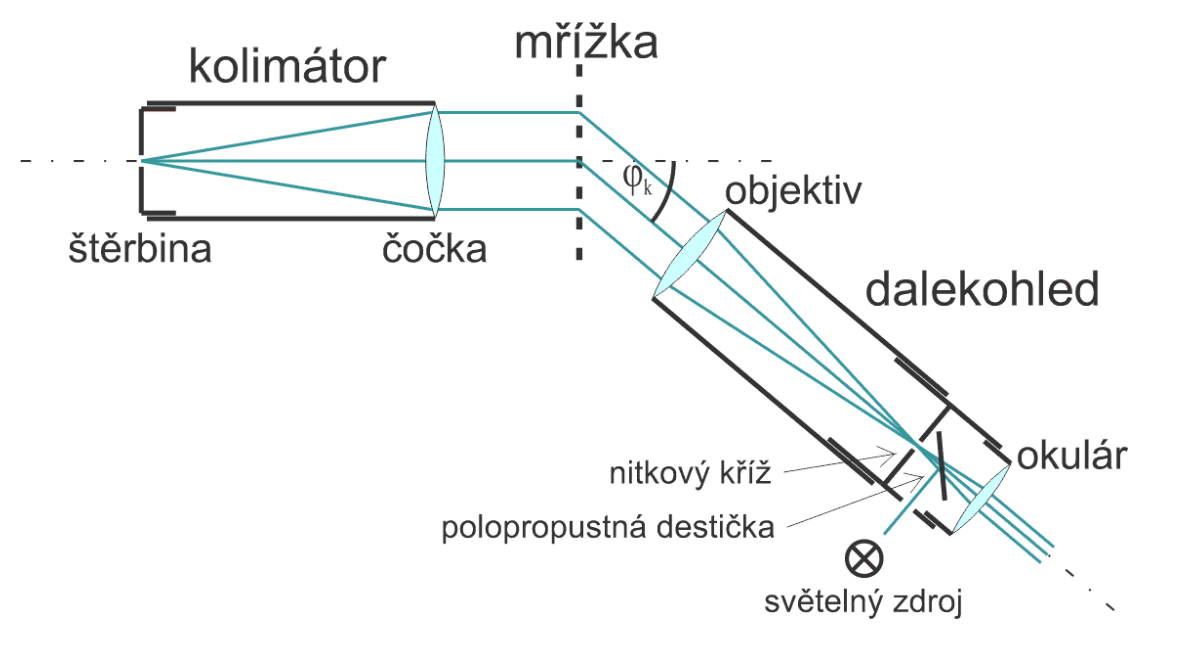
\includegraphics[width=0.5\linewidth]{spektrometr.png}
    \caption{Schéma mřížkového spektrometru \cite{pokyny}}
    \label{sch:spektrometr}
\end{schema}


\subsection{Měřicí přístroje a jejich nejistoty}
\begin{enumerate}
    \item Goniometr:
    
    Goniometrem byl měřen úhel natočení dalekohledu. Při nastavení
    nitkového kříže na určitou spektrální čáru byl takto měřen úhel
    odklonu $\varphi_k$ světla od původního směru šíření. Stupnice
    goniometru umožnovala odečítat úhly s přesností na $1\,\mathrm{'}$,
    dílky nonia a hlavní stupnice však nepřiléhaly těsně k sobě, 
    což ztěžovalo přesné odečítání. Proto odhaduji nejistotu měření
    úhlu jako $\sigma_\varphi = 3\,\mathrm{'}$.

\end{enumerate}


% ======================== VÝSLEDKY MĚŘENÍ ===========================
\section{Výsledky měření}

\subsection{Určení mřížkové konstanty}
Nejprve bylo proměřováno spektrum sodíkové výbojky, konkrétně čáry
sodíkového dubletu o vlnových délkách $\lambda_{D1} = \qty{589.0}{nm}$
a $\lambda_{D2} = \qty{589.6}{nm}$ \cite{pokyny}, a to pro 1.
a 2. řád. Měření bylo provedeno na obou stranách od hlavního maxima,
nalevo byl změřen úhel $\psi_1$ a napravo úhel $\psi_2$. Úhel
$\varphi_k$ byl vypočten jako polovina vzdálenosti těchto dvou úhlů,
se započítáním korekce kvůli nepříliš vhodně zvolené stupnici
(jež obsahuje skok o $360\degree$ v okolí základní pozice dalekohledu):
\begin{equation}\label{phik}
    \varphi_k = \frac{\psi_1 - \left(\psi_2 - 360^\circ\right)}{2} \, .
\end{equation}

V tabulce \ref{tab:sodik} jsou uvedeny naměřené úhly pro sodíkový 
dublet pro oba řády a jim odpovídající mřížkové konstanty vypočtené 
z rovnice (\ref{mrizka}). Nejistota úhlu $\varphi_k$ byla určena
podle \cite{englich} jako
\begin{equation}\label{sigmaphik}
    \sigma_{\varphi_k} = \frac{\sqrt{2}}{2}\sigma_{\psi} 
\end{equation}
a nejistota mřížkové konstanty vypočtené pomocí rovnice 
(\ref{mrizka}) jako
\begin{equation}\label{sigmaa}
    \sigma_a = a \sigma_{\varphi_k} \tan \varphi_k \, ,
\end{equation}
přičemž uvažuji, že nejistoty vlnových délek jsou zanedbatelné
oproti nejistotě úhlu $\varphi_k$.

\begin{table}[!htbp]
\centering
\caption{Naměřené úhly maxim 1. a 2. řádu sodíkového dubletu a
vypočtené mřížkové konstanty.}
\begin{tabular}{cccccc}
 \toprule
 $k$ & $\lambda_\mathrm{Na}$ (nm) & $\psi_1$ (°) & $\psi_2$ (°) & $\varphi_k$ (°) & $a$ (nm) \\
 \midrule
 $1$ & $589.0$ & $21.78(5)$ & $340.12(5)$ & $20.83(4)$ & $1656.1(4)$ \\
 $1$ & $589.6$ & $21.85(5)$ & $340.05(5)$ & $20.90(4)$ & $1652.8(4)$ \\
 $2$ & $589.0$ & $46.80(5)$ & $316.17(5)$ & $45.32(4)$ & $1656.8(10)$ \\
 $2$ & $589.6$ & $46.87(5)$ & $316.05(5)$ & $45.41(4)$ & $1655.9(10)$ \\
 \bottomrule
\end{tabular}
\label{tab:sodik}
\end{table}

Průměrná mřížková konstanta byla vypočtena jako vážený průměr
mřížkových konstant, kde váhami jsou převrácené druhé mocniny
jejich standardních nejistot:
\begin{equation}\label{abar}
    \bar{a} = \frac{\sum_{n=1}^{4}\frac{a_i}{\sigma_{a_i}^2} }{\sum_{n=1}^{4}\frac{1}{\sigma_{a_i}^2}} \, .
\end{equation}
Její nejistota byla určena podle \cite{englich} jako
\begin{equation}\label{sigmaabar}
    \sigma_{\bar{a}} = \frac{1}{\sqrt{\sum_{n=1}^{4}\frac{1}{\sigma_{a_i}^2}}} \, .
\end{equation}

Průměrná mřížková konstanta tedy vychází $\bar{a} = 1654.7(3)\,\mathrm{nm}$,
čemuž odpovídá počet vrypů na jednotku délky $N = 604.3(1)\,\mathrm{mm^{-1}}$. Nejistotu
$N$ jsem určil podle \cite{englich} jako
\begin{equation}\label{sigmaN}
    \sigma_N = N \relative{\bar{a}} \, .
\end{equation}

\subsection{Rozlišovací schopnost}

Pro první řád čar sodíkového dubletu uvažuji, že lze nejvýše rozlišit právě tyto dvě vlnové délky, tedy
\\ $\delta \lambda_1 = \qty{0.6}{nm}$. Na~druhém řádu jsou již čáry ve větší vzdálenosti od sebe, proto odhaduji,
že lze rozlišit i poloviční rozdíl vlnových délek, tedy $\delta \lambda_2 = \qty{0.3}{nm}$. Podle vztahu
(\ref{rozliseni}) tedy experimentální rozlišovací schopnost pro první řád vychází $R_1 = 1.0(1) \cdot 10^2$
a pro druhý řád $R_2 = 2.0(2) \cdot 10^3$. Nejistoty jsem určil pomocí relativní nejistoty rozdílu $\delta \lambda$,
kterou odhaduji jako $10 \, \%$:
\begin{equation}\label{sigmaR}
    \sigma_R = R \relative{\delta \lambda} \, .
\end{equation}

Maximální teoretická rozlišovací schopnost (daná čistě vlnovými vlastnostmi světla) byla určena pomocí vztahu 
(\ref{maxrozliseni}) a (\ref{m}), přičemž jsem uvažoval $D = \qty{18}{mm}$ a $a = 1654.7(3)\,\mathrm{nm}$.
Pro první řád tak vychází \\ $R_{m1} = 8920(1)$ a pro druhý řád $R_{m2} = 17840(3)$.
Nejistoty jsem určil z relativní nejistoty mřížkové konstanty $a$ jako
\begin{equation}\label{sigmaRm}
    \sigma_{R_m} = R_m \relative{a} \, .
\end{equation}
Maximální teoretická rozlišovací schopnost je tedy řádově větší než rozlišovací
schopnost určená experimentálně, odůvodnění v Diskuzi.

\subsection{Spektrální čáry rtuti}

Obdobným způsobem jako se sodíkovou výbojkou byly proměřeny spektrální čáry rtuti, ovšem jen pro řád $k=1$.
V tabulce \ref{tab:rtut} jsou uvedeny naměřené úhly $\psi_1$ a $\psi_2$,
vypočtené střední úhly $\varphi_1$ a také vlnové délky, a to experimentálně určené
pomocí rovnice (\ref{mrizka}) i tabulkové hodnoty z \cite{tabulka}. Uvedena
je i druhá modrozelená čára, která byla ve spektru zřetelná, přestože ji
tabulka \cite{tabulka} nezmiňuje. Nejistota experimentálně vypočtené vlnové
délky byla určena podle \cite{englich} jako
\begin{equation}\label{sigmalambda}
    \sigma_{\lambda_\mathrm{Hg}} = \lambda_\mathrm{Hg} \sqrt{\relsqr{a} + \squared{\frac{\sigma_{\varphi_1}}{\tan \varphi_1}}} \, .
\end{equation}
Nejistotu tabelované vlnové délky jsem neuvažoval.

\begin{table}[!htbp]
\centering
\caption{Spektrální čáry rtuti}
\begin{tabular}{cccccc}
 \toprule
 barva & $\psi_1\, (\mathrm{\degree})$ & $\psi_2\, (\mathrm{\degree})$ & $\varphi_1\, (\mathrm{\degree})$ & $\lambda_\mathrm{Hg}\, (\mathrm{nm})$ & $\lambda_\mathrm{tab}\, (\mathrm{nm})$ \\
 \midrule
 fialová & $14.88(5)$ & $346.57(5)$ & $14.16(4)$ & $405(1)$ & $405$ \\
 fialová & $14.93(5)$ & $346.43(5)$ & $14.25(4)$ & $407(1)$ & $408$ \\
 modrá & $15.93(5)$ & $345.53(5)$ & $15.20(4)$ & $434(1)$ & $434$ \\
 modrá & $15.95(5)$ & $345.48(5)$ & $15.23(4)$ & $435(1)$ & $435$ \\
 modrá & $15.98(5)$ & $345.45(5)$ & $15.27(4)$ & $436(1)$ & $436$ \\
 modrozelená & $17.98(5)$ & $343.57(5)$ & $17.21(4)$ & $490(1)$ & $492$ \\
 modrozelená & $18.18(5)$ & $343.35(5)$ & $17.42(4)$ & $495(1)$ &  \\
 zelená & $19.97(5)$ & $341.55(5)$ & $19.21(4)$ & $544(1)$ & $546$ \\
 žlutá & $21.08(5)$ & $340.37(5)$ & $20.36(4)$ & $576(1)$ & $577$ \\
 žlutá & $21.18(5)$ & $340.30(5)$ & $20.44(4)$ & $578(1)$ & $579$ \\
 červená & $22.22(5)$ & $339.32(5)$ & $21.45(4)$ & $605(1)$ & $607$ \\
 červená & $22.42(5)$ & $339.17(5)$ & $21.62(4)$ & $610(1)$ & $612$ \\
 červená & $22.82(5)$ & $338.75(5)$ & $22.03(4)$ & $621(1)$ & $623$ \\
 červená & $24.65(5)$ & $336.82(5)$ & $23.92(4)$ & $670.8(9)$ & $672$ \\
 červená & $25.48(5)$ & $336.20(5)$ & $24.64(4)$ & $689.9(9)$ & $691$ \\
 \bottomrule
\end{tabular}
\label{tab:rtut}
\end{table}

\subsection{Kalibrační křivka a rezidua}

Kalibrační křivka byla vytvořena podle pokynů \cite{pokyny} jako závislost
tabelované vlnové délky $\lambda_\mathrm{tab}$ (z \cite{tabulka}) na měřeném úhlu $\varphi_1$.
Křivka je vykreslena v grafu \ref{fig:kalibrace}. Při zpracování dat přímo v laboratoři
byla datovými body proložena lineární závislost. Z grafu reziduí však bylo patrné,
že rozdíl mezi daty a kalibrační křivkou není náhodný, ale vykazuje zřejmou
kvadratickou závislost. Proto byla kalibrační křivka následně proložena
kvadratickou funkcí $\lambda_\mathrm{tab} = A \varphi_1^2 + B \varphi_1 + C$.
Koeficienty byly určeny s pomocí knihovny \texttt{numpy.Polynomial} váženou lineární regresí,
přičemž váhou byly převrácené druhé mocniny nejistoty úhlu $\varphi_1$. Jejich
hodnoty shrnuje tabulka \ref{tab:koeficienty}.

Graf reziduí mezi daty a kalibrační křivkou je pak zobrazen v grafu
\ref{fig:rezidua}. I těmito datovými body byla proložena kvadratická funkce,
její koeficienty však neuvádím, protože jsou všechny triviálně nulové.

\begin{table}[!htbp]
\centering
\caption{Koeficienty kalibrační křivky}
\begin{tabular}{ccc}
 \toprule
 $A\, (\mathrm{nm\,/\, \degree^{2}})$ & $B\, (\mathrm{nm\,/\, \degree})$ & $C\, (\mathrm{nm})$ \\
 \midrule
 $-0.1(7)$ & $30(1)$ & $-9.9(12)$ \\
 \bottomrule
\end{tabular}
\label{tab:koeficienty}
\end{table}

\begin{figure}
    \centering
    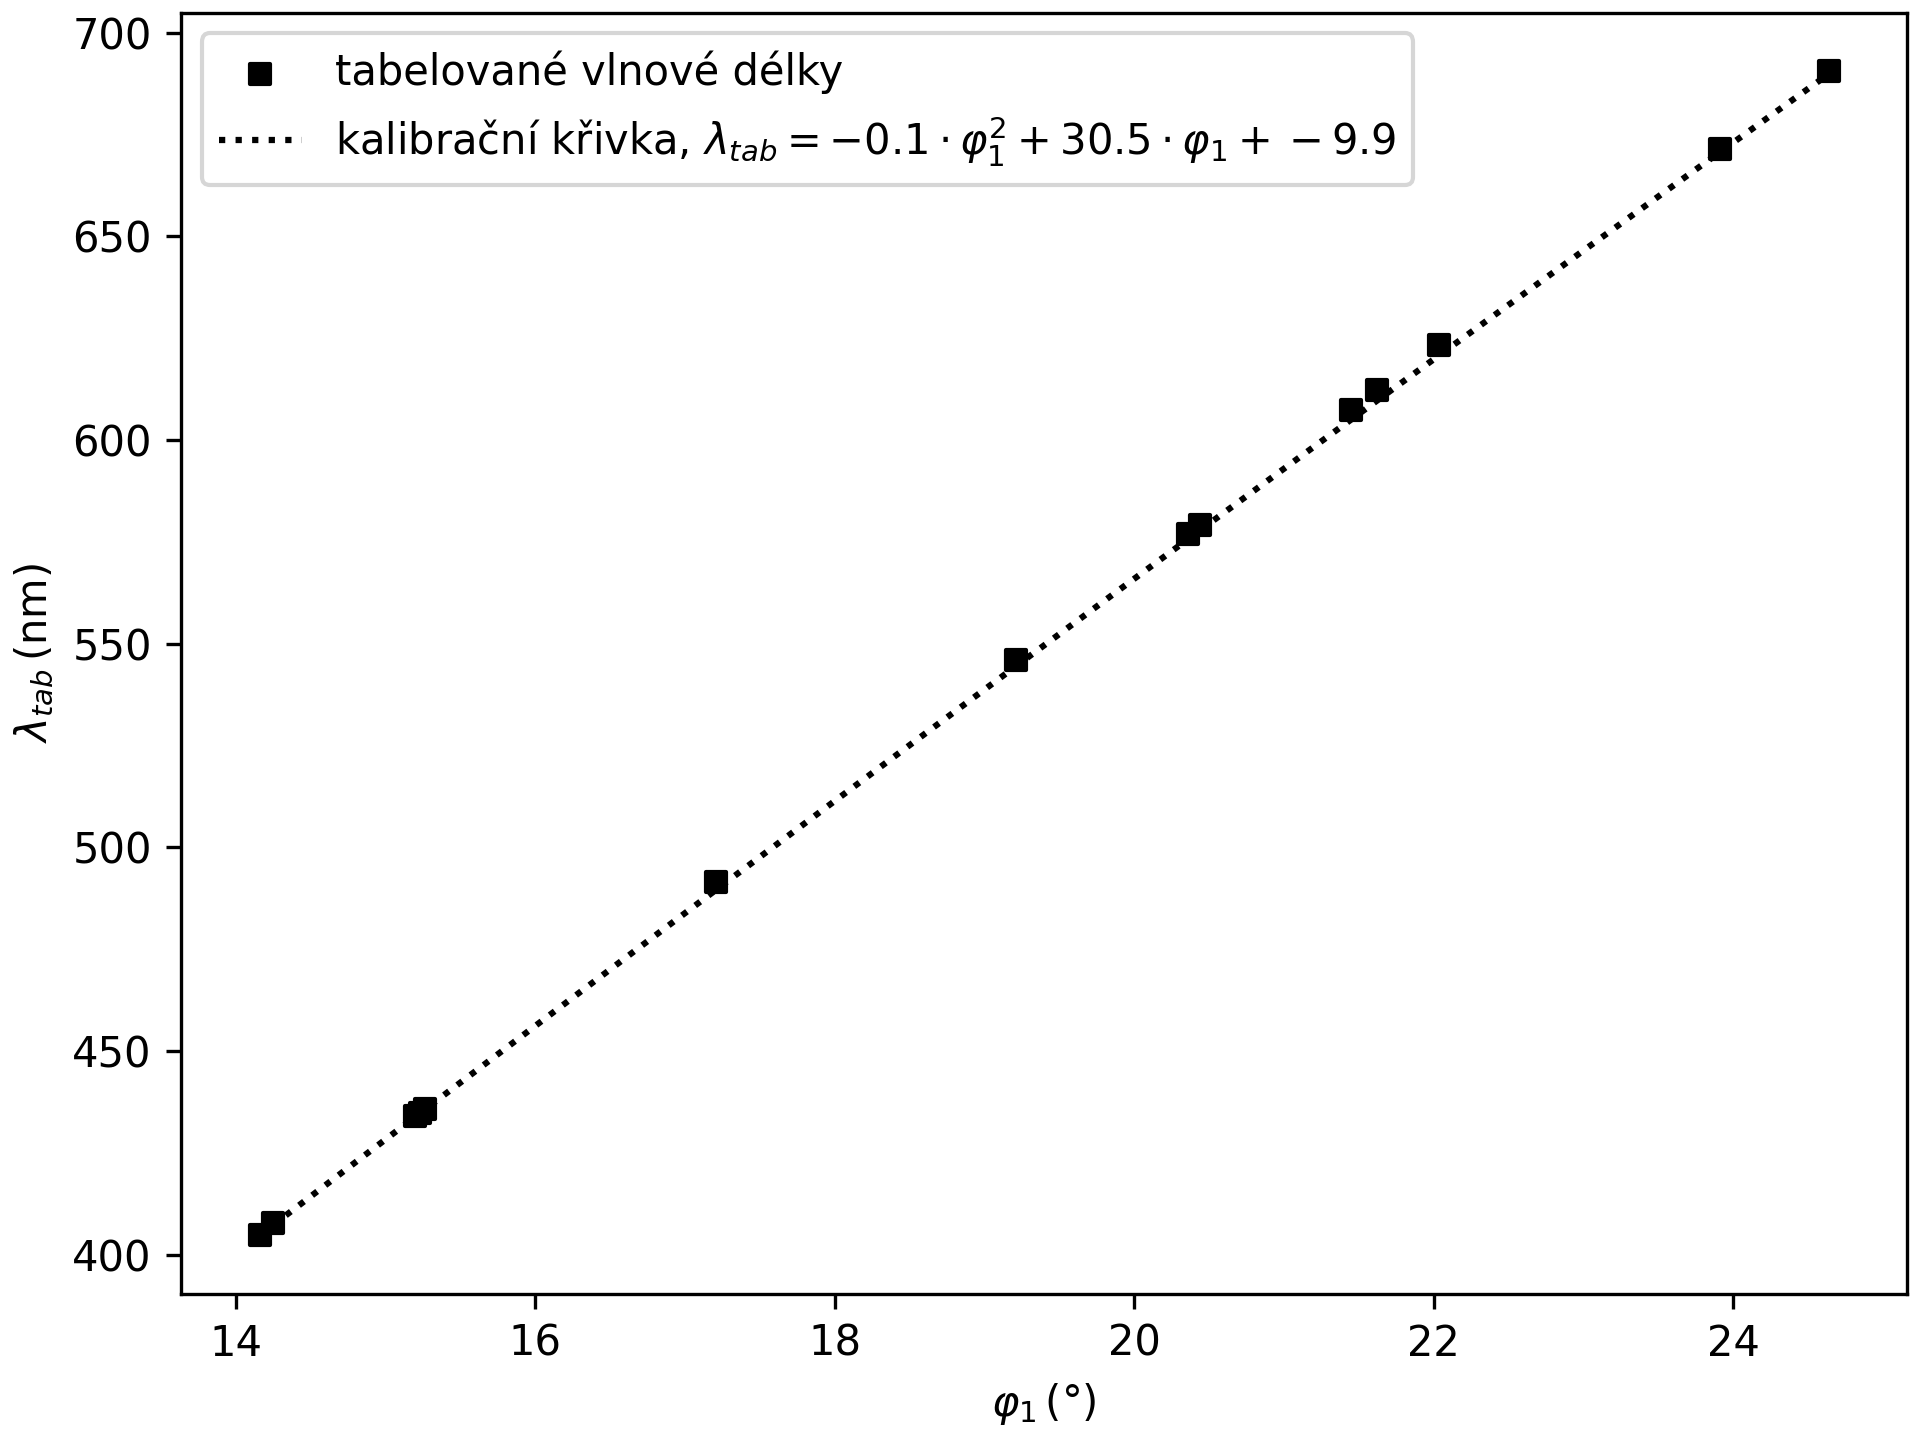
\includegraphics[width=0.7\linewidth]{calibration.png}
    \caption{Kalibrační křivka pro vlnové délky rtuti. \nobars}
    \label{fig:kalibrace}
\end{figure}

\begin{figure}
    \centering
    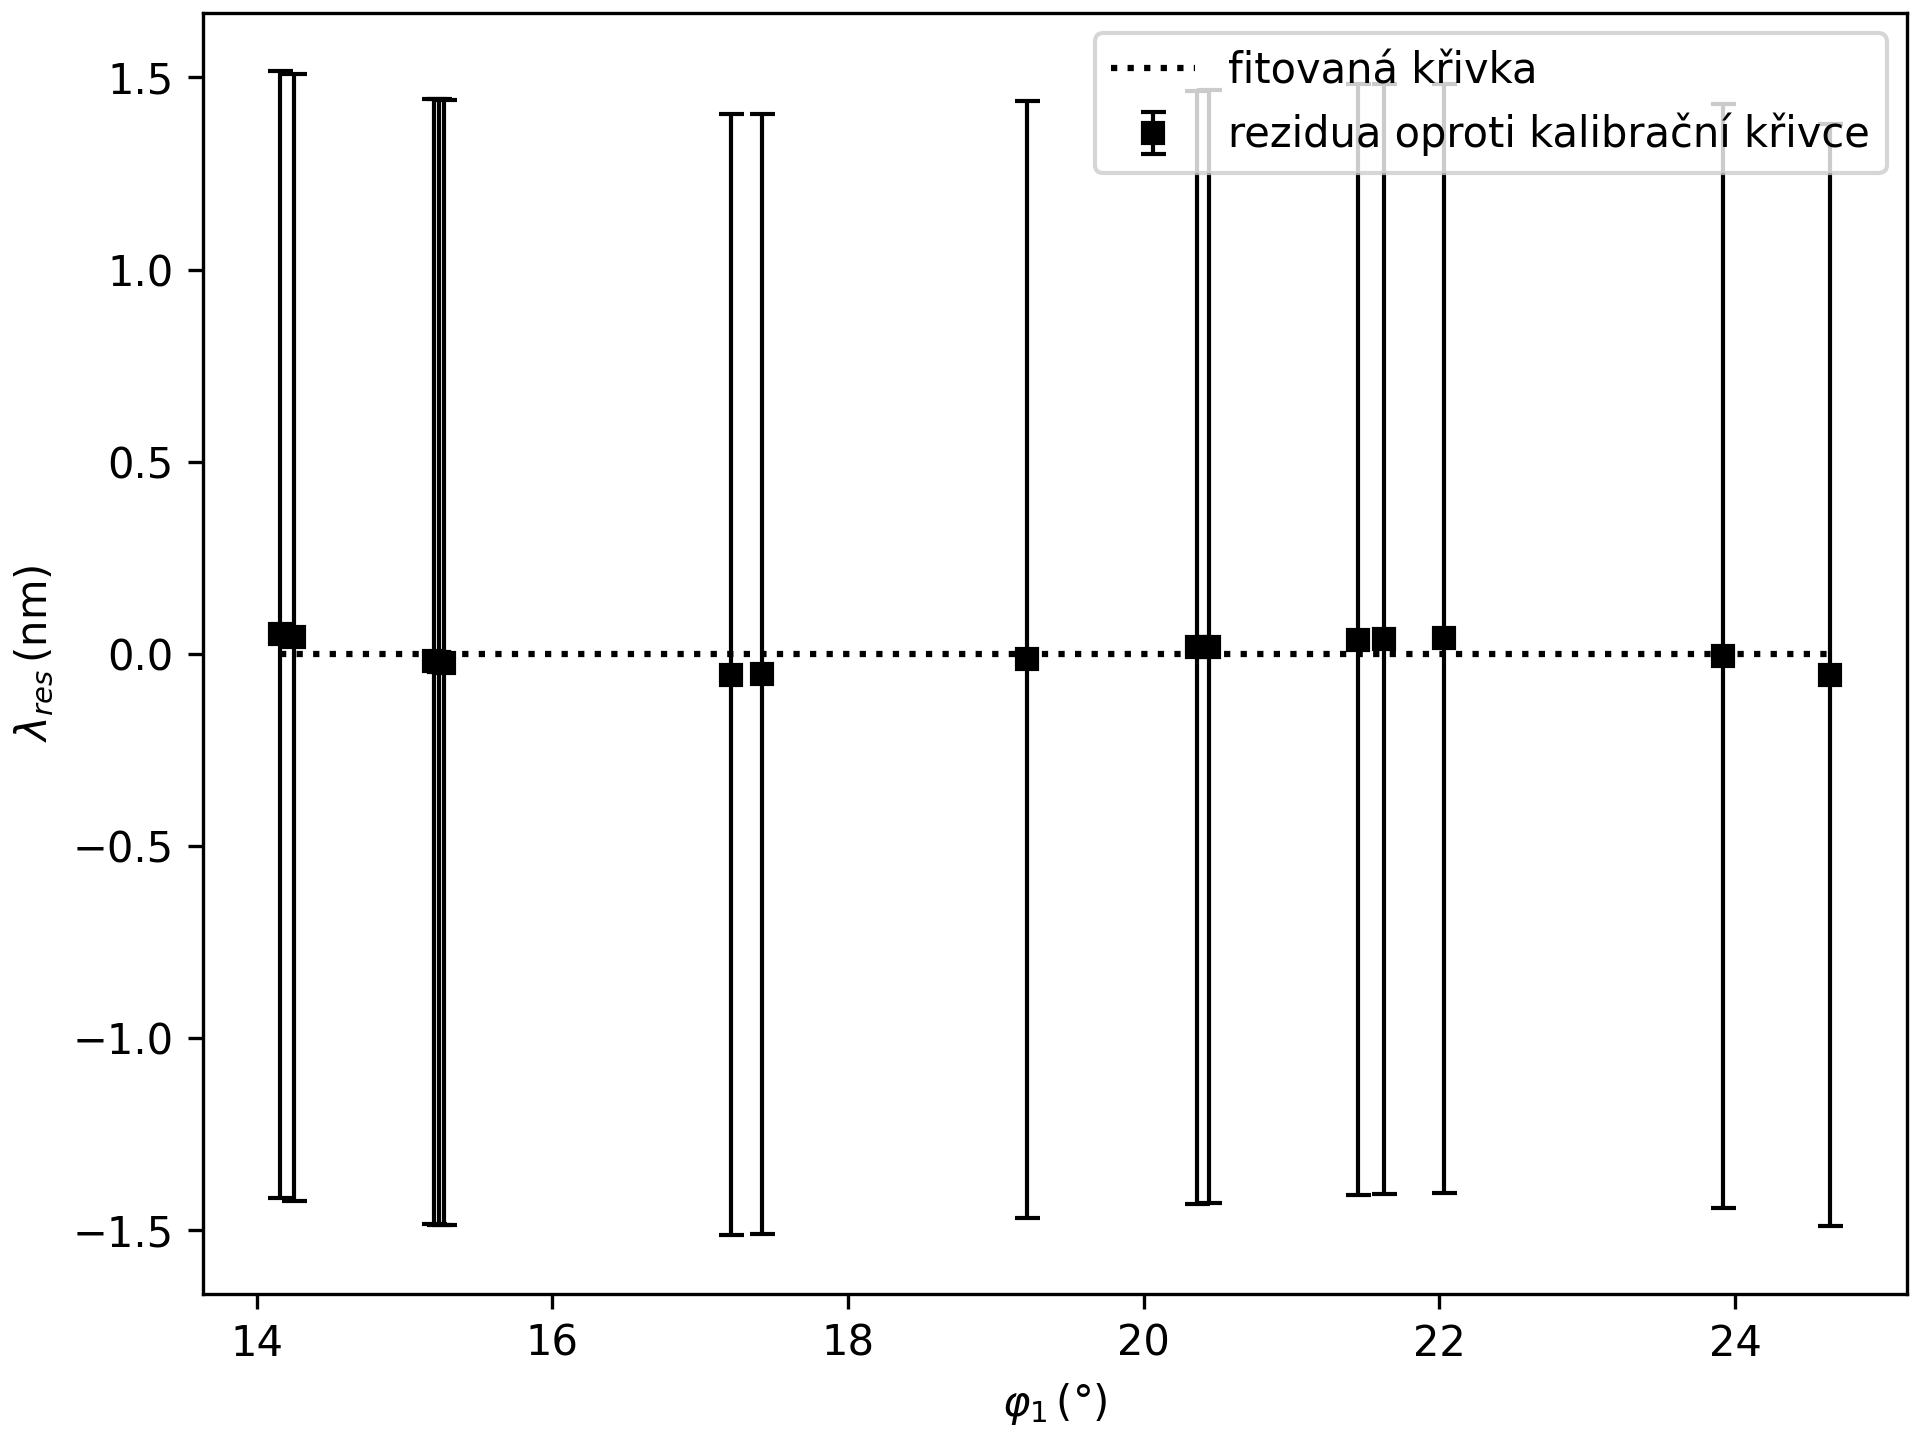
\includegraphics[width=0.7\linewidth]{residuals.png}
    \caption{Rezidua mezi naměřenými vlnovými délkami a kalibrační křivkou.}
    \label{fig:rezidua}
\end{figure}

\subsection{Úhlová disperze}

Pro 1. a 2. řád spektra sodíku a 1. řád spektra rtuti byla určena úhlová
disperze mřížky, a to jednak experimentálně pomocí vztahu (\ref{disperzeexp})
ze sousedních žlutých čar, jednak teoreticky pomocí vzorce (\ref{disperzeteor}),
kde úhel $\varphi_k$ je úhel mezi těmito dvěma čarami. Nejistota
experimentální úhlové disperze byla určena podle \cite{englich} jako
\begin{equation}\label{sigmaDe}
    \sigma_{D_{ae}} = D_{ae} \sqrt{\relsqr{\Delta \varphi_k} + \relsqr{\Delta \lambda}} \, ,
\end{equation}
kde $\Delta \varphi_k$ je rozdíl úhlů mezi dvěma sousedními žlutými čarami
a $\Delta \lambda$ je rozdíl jejich vlnových délek. Pro~ nejistotu
$\Delta \varphi_k$ platí $\sigma_{\Delta \varphi_k} = \sqrt{2}\,\sigma_{\varphi_k}$
Pro výpočet hodnoty i nejistoty
úhlové disperze bylo nutné pracovat s úhly v radiánech. U sodíku je relativní nejistota
rozdílu vlnových délek zanedbatelná oproti relativní nejistotě rozdílu úhlů,
u rtuti jsou však srovnatelné.
Nejistota teoretické úhlové disperze byla určena podle \cite{englich} jako
\begin{equation}\label{sigmaDt}
    \sigma_{D_{at}} = D_{at} \sqrt{\relsqr{a} + {\sigma^2_{\varphi_k}\tan^2 \varphi_k}} \, .
\end{equation}

Vypočtené hodnoty úhlových disperzí shrnuje tabulka \ref{tab:disperze}.

\begin{table}[!htbp]
\centering
\caption{Úhlová disperze mřížky pro 1. a 2. řád spektra sodíku a 1. řád spektra rtuti.}
\begin{tabular}{cccc}
 \toprule
 prvek & k & $D_{ae}\, (\mathrm{mm^{-1}})$ & $D_{at}\, (\mathrm{mm^{-1}})$ \\
 \midrule
 Na & 1 & $1.9(15)\cdot 10^3$ & $646.77(15)$ \\
 Na & 2 & $2.7(15)\cdot 10^3$ & $860.1(4)$ \\
 Hg & 1 & $6(5)\cdot 10^2$ & $644.79(14)$ \\
 \bottomrule
\end{tabular}
\label{tab:disperze}
\end{table}

% ============================ DISKUZE ===============================
\section{Diskuze}

Spektrální čáry sodíku i rtuti byly proměřovány na obou stranách od hlavního
maxima, aby se vyloučila systematická chyba nenulového úhlu $\varphi_0$.
Při měření úhlů na obou stranách a vypočtení jejich vzdálenosti (jejich rozdílu)
se tím totiž případný posun $\varphi_0 \neq 0$ odečte. Nejvýhodnější by bylo
uvažovat úhlovou stupnici s nulou v pozici hlavního maxima, kdy by byly
úhly na obou stranách navzájem opačné. Stupnice goniometru měla hodnoty
od 0\degree do 360\degree, proto bylo nutné při výpočtu výsledného úhlu $\varphi_k$
provést korekci o 360\degree, vizte vztah (\ref{phik}).

Proměřováním spektra sodíku byla určena mřížková konstanta $a = 1654.7(3)\,\mathrm{nm}$,
které odpovídá počet vrypů na jednotku délky $N = 604.3(1)\,\mathrm{mm^{-1}}$
s relativní nejistotou $0.2\,\%$. Tato hodnota se v rámci nejistoty neshoduje
s udávanou hodnotou $N = 600\,\mathrm{mm^{-1}}$ na mřížce, řádově si však
odpovídají. Odhaduji proto, že byla buď stále ještě podceněna nejistota
určení úhlu na goniometru, nebo že přístroj nebyl zcela správně seřízen
a meření tak je ovlivněno systematickou chybou.

Rozlišovací schopnosti určené na základě vzdálenosti čar sodíkového dubletu
$R_1 = 1.0(1) \cdot 10^2$ a \\ $R_2 = 2.0(2) \cdot 10^2$
(s relativní nejistotou $10\,\%$) jsou řádově menší
než maximální teoretické hodnoty $R_{m1} = 8920(1)$ a $R_{m2} = 17840(3)$
(s relativní nejistotou $0.02\,\%$).
Architektura spektrometru je tedy zřejmě více omezující než čistě vlnové 
vlastnosti světla. Odhaduji, že hlavní roli hraje rozlišení a zvětšení
dalekohledu. Pokud by čáry byly ostřejší a pozorovatelné pod větším
zorným úhlem, bylo by možné experimentálně rozlišit i menší rozdíl vlnových
délek. Rozlišovací schopnost pro druhý řád je vyšší než pro první řád,
protože čáry jsou od sebe v~důsledku rovnice (\ref{mrizka}) více vzdálené.

Vlnové délky spektrálních čar rtuti se podařilo určit s relativní nejistotou
v řádu desetin procent, přičemž se v~rámci nejistot (nebo v rámci $2 \sigma_{\lambda_\mathrm{Hg}}$)
shodují s uvedenými tabelovanými hodnotami. Některé čáry, především ty
v~červené oblasti spektra, byly obtížně viditelné, vzhledem ke shodě s tabulkovými
hodnotami však předpokládám, že se jedná o správné čáry a ne o artefakty
způsobené např. odrazem nějaké jasnější čáry v~přístroji.

Závislost tabelované vlnové délky na úhlu $\varphi_1$ lze dobře popsat
kvadratickou závislostí, jak ukazuje graf \ref{fig:kalibrace}. Koeficient
lineárního členu je větší než koeficient kvadratického členu a na první pohled
by se mohlo lineární proložení dat zdát vyhovující. Z grafu reziduí mezi
naměřenými vlnovými délkami a kalibrační křivkou je však zřejmé, že 
závislost vlnové délky na úhlu je minimálně kvadratická. Při proložení dat
pouze lineární funkcí totiž vykazovala rezidua zjevnou kvadratickou závislost.
Takto jsou rezidua v rámci nejisot náhodně rozmístěna kolem nuly (polynom stupně
2, jímž byla rezidua proložena, je dokonce triviálně nulový). Odhaduji proto,
že přesnost kalibrace dat je v rámci nejistot měření dostatečná.

Úhlová disperze mřížky určená ze žlutých spektrálních čar sodíku vychází pro první
řád $D^\mathrm{Na\,1}_{ae} = 1.9(15)\cdot 10^3\, \mathrm{mm^{-1}}$ s relativní
nejistotou $80\,\%$ a pro druhý řád $D^\mathrm{Na\,2}_{ae} = 2.7(15)\cdot 10^3\, \mathrm{mm^{-1}}$
s relativní nejistotou $56\,\%$. Pro~rtuť je úhlová disperze 
$D^\mathrm{Hg\,1}_{ae} = 6(5)\cdot 10^2\, \mathrm{mm^{-1}}$ s relativní
nejistotou $80\,\%$.
Takto vysoké nejistoty jsou způsobeny zejména
vysokou relativní nejistotou rozdílu úhlů mezi dvěma sousedními čarami. Pro 
rtuť je významná i~relativní nejistota rozdílu vlnových délek,
která je však také daná nejistotou měření úhlů.
Teoretické hodnoty úhlové disperze vypočtené z rovnice (\ref{disperzeteor})
jsou pro sodík menší než experimentální, pro rtuť si hodnoty odpovídají.
V rámci nejistot se všechny hodnoty shodují, přesnost měření však není
dostatečná, aby bylo možné jejich shodu potvrdit. Pro větší přesnost měření
by bylo nutné pracovat s přesnějším goniometrem, který by umožňoval odečítat
úhly s menší nejistotou. Teoretické hodnoty byly určeny s větší přesností
než experimentální (relativní nejistota v řádu setin až desetin procent),
neboť jsou dány pouze mřížkovou konstantou $a$ a úhlem $\varphi_k$ a nikoliv
rozdílem dvou blízkých hodnot úhlů nebo vlnových délek.

% ============================= ZÁVĚR ================================
\section{Závěr}

Mřížková konstanta byla určena jako $a = 1654.7(3)\,\mathrm{nm}$, 
což odpovídá počtu vrypů na jednotku délky \\ $N = 604.3(1)\,\mathrm{mm^{-1}}$.

Rozlišovací schopnost určená experimentálně z čar sodíkového dubletu
vychází pro první ($R_1$) a druhý ($R_2$) řád jako
\begin{equation*}
    R_1 = 1.0(1) \cdot 10^2
\end{equation*}
\begin{equation*}
    R_2 = 2.0(2) \cdot 10^2 \, .
\end{equation*}
Maximální teoretické rozlišovací schopnosti jsou však
\begin{equation*}
    R_{m1} = 8920(1)
\end{equation*}
\begin{equation*}
    R_{m2} = 17840(3) \, .
\end{equation*}

Naměřené vlnové délky spektrálních čar rtuti se v rámci nejistot shodují
s tabelovanými hodnotami. Jejich závislost na úhlu $\varphi_1$ lze dobře
popsat kvadratickou závislostí, avšak s dominantním lineárním členem.

Úhlová disperze mřížky vypočtená z čar ve žluté oblasti spektra sodíku
vychází pro první řád 
\begin{equation*}
    D^\mathrm{Na\,1}_{ae} = 1.9(15)\cdot 10^3\, \mathrm{mm^{-1}} \, ,
\end{equation*}
přičemž teoretická hodnota činí
\begin{equation*}
    D^\mathrm{Na\,1}_{at} = 646.77(15)\, \mathrm{mm^{-1}}
\end{equation*}
a pro druhý řád
\begin{equation*}
    D^\mathrm{Na\,2}_{ae} = 2.7(15)\cdot 10^3\, \mathrm{mm^{-1}} \, ,
\end{equation*}
s teoretickou hodnotou
\begin{equation*}
    D^\mathrm{Na\,2}_{at} = 860.1(4)\, \mathrm{mm^{-1}} \, .
\end{equation*}
Pro první řád spektra rtuti byla spočtena experimentální úhlová disperze
\begin{equation*}
    D^\mathrm{Hg\,1}_{ae} = 6(5)\cdot 10^2\, \mathrm{mm^{-1}} \, ,
\end{equation*}
a teoretická je
\begin{equation*}
    D^\mathrm{Hg\,1}_{at} = 644.79(14)\, \mathrm{mm^{-1}} \, .
\end{equation*}

% =========================== LITERATURA =============================
\begin{thebibliography}{9}

\bibitem{pokyny} Kolektiv ZFP KVOF MFF UK: Mřížkový spektrometr [online]. [cit. 24.2.2026], dostupné
z~https://physics.mff.cuni.cz/vyuka/zfp/\_media/zadani/pokyny/mereni\_303.pdf

\bibitem{englich} J. Englich: Úvod do praktické fyziky I: Zpracování výsledků měření. 1. vyd. Praha: Matfyzpress, 2006

\bibitem{tabulka} Kolektiv ZFP KVOF MFF UK: Tabulka spektrálních čar rtuti,
přiložená k pokynům u úlohy.


\end{thebibliography}
\end{document}
